\documentclass[tikz,border=2mm]{standalone}

\usepackage{bm}
\usepackage{xcolor}
\usetikzlibrary{arrows,positioning}
\usetikzlibrary{arrows.meta}

\begin{document}

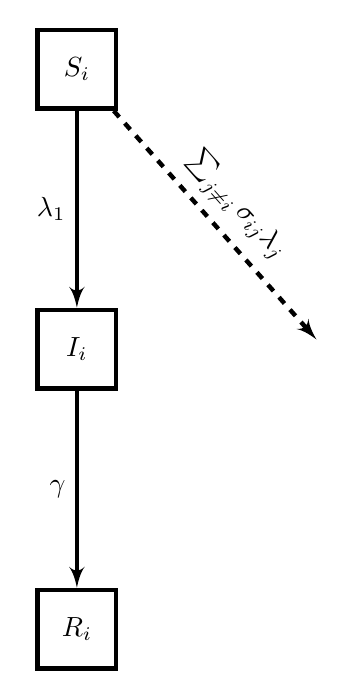
\begin{tikzpicture}[node distance=2.5cm,auto,>=latex',every node/.append style={align=center},int/.style={draw, minimum size=1cm},inverter/.style={rectangle,draw,inner sep=2pt,minimum size=6mm},posnode/.style={shape=rectangle, draw=orange, line width=2},
  negnode/.style={shape=rectangle, draw=black, line width=2}]
    \node [int, ultra thick] (S1)             {$S_i$};
    \node [int, below=of S1, ultra thick] (I1)             {$I_i$};
    \node [right=of I1] (tmp)             {};
    \node [int, below=of I1, ultra thick] (R1)             {$R_i$};
    \path[->, ultra thick, left] (S1) edge node {$\lambda_1$} (I1);
    \path[->, ultra thick, above, sloped, dashed] (S1) edge node {$\sum_{j \neq i} \sigma_{ij} \lambda_j$} (tmp);
    \path[->, ultra thick, left] (I1) edge node {$\gamma$} (R1);
\end{tikzpicture}
\end{document}
